\section{Performance of a detector}


\subsection{Signal response}

A particle is detected if it passes through our detector and leaves some
energy behind. These detections end up as a digitized list of numbers
with a timestamp. However, before a particle signal ends up in its
digital form it passes through the various parts of the detector. Not
all parts perfectly transport the particle signal. These effects, which
prevent the detector from having perfect timing and particle counting
will be outlined. These also serve as probability distributions that are
used in detector simulations.


\subsection{Energy loss}

Particles loose energy in the detector because of interactions with the
polyvinyltoluene in the scintillator. Ionization and Bremsstrahlung and
the main sources of energy loss for energetic charged particles
(electrons, muons). The scintillator is \SI{2}{\centi\meter} thick, if
particles enter de detector they may have a longer path in the detector.
It can also be shorter if the particle passes through one of the edges
of the scintillator, however, due to the large area of the detector the
chance of that happening is relatively low. The amount of energy
deposited by the particle going through the detector is described by the
Bethe-Bloch formula. This formula gives the stopping power, the amount
of energy lost by the particle per \SI{}{\gram\centi\meter\square} of
the material it passes through. However, the interactions in which the
particles loose energy is a statistical process, so the energy loss is
not a fixed number but a distribution. (figure...)

Energetic photons can also deposit energy in the scintillator due to
Compton scattering and pair creation. However, the cross sections for
these interactions is very low. A \SI{1}{\mega\electronvolt} photon  has
a mean free path greater than \SI{10}{\centi\meter}, which increases
further for higher energy photons, see fig [By Jos/Tom]. Despite the low
detection chance, the large number of photons in an air shower makes
them statistically relevant.

According to the specifications the amount of light produced in a
scintillator as a function of temperature should be constant between
\SI{-60}{\degreeCelsius} and \SI{20}{\degreeCelsius}. At
\SI{60}{\degreeCelsius} the light output is decreased by
\SI{5}{\percent} relative to the output at \SI{20}{\degreeCelsius}.
Temperature in a skibox can rise above the local outside temperature
when the sun shines upon it. Temperature loggers have measured
differences of over \SI{10}{\degreeCelsius} above the local outside
temperature. Rarely but sometimes the temperature in the Netherlands can
reach \SI{40}{\degreeCelsius}, so on such occasions the efficiency fo
the scintillator might be \SI{3.75}{\percent} below nominal. Given the
rare occurrence of such extremely high temperatures and the small effect
this is ignored in the simulations.


\subsection{Light transmission}

Because of the geometry of the detector the position of the scintillator
that the particle goes through is significant. The light emitted along
the path of the particle is transmitted in random directions. Depending
on the angle at which the emitted photons hit the outer edges of the
scintillator there is a chance that they will be reflected back or leave
the scintillator. The entire detector is wrapped in aluminium foil 
to reflect those photons back into the scintillator. To
detect the photons they need to hit the windows of \pmt. To get to the
\pmt they need to pass from the scintillator through a layer of optical
glue, the light guide, another layer of optical glue, a small piece of
light guide, and finally a layer of optical tape to reach the \pmt.
During this many photons will be reflected a number of times. For
\SI{1}{\mip} approximately 30000 photons [check.] are emitted, most will
not make it to the \pmt.

A 2D Monte Carlo simulation performed by Jos Steijger which tracked
photons from emission until they either reach the \pmt or leave the
detector (ignoring the aluminium foil) gives transmission efficiency
information at any location in the scintillator.

Coincidence tests using a small (\SI[product-units = repeat]{1 x
1}{\centi\meter}) scintillator with a \pmt and a normal \hisparc
detector provided verification of this simulation. By moving the small
detector over the large scintillator they will also trigger on single
muons passing through both detectors. This makes it possible to check
the efficiency at a specific point of the detector.

In the simulations we use the Bethe Bloch, energy straggling, Landau
distribution convoluted with the efficiency modelled by Jos as
distribution which can be scaled by cosine of angle of incidence.

\begin{figure}
    \centering
    % \usepackage{tikz}
% \usetikzlibrary{arrows}
% \usepackage{pgfplots}
% \pgfplotsset{compat=1.3}
% \usepackage[detect-family]{siunitx}
% \usepackage[eulergreek]{sansmath}
% \sisetup{text-sf=\sansmath}
% \usepackage{relsize}
%
\tikzsetnextfilename{externalized-signal_efficiency}
\pgfkeysifdefined{/artist/width}
    {\pgfkeysgetvalue{/artist/width}{\defaultwidth}}
    {\def\defaultwidth{ .67\linewidth }}
%
%
\begin{sansmath}
\begin{tikzpicture}[
        font=\sffamily,
        every pin/.style={inner sep=2pt, font={\sffamily\smaller}},
        every label/.style={inner sep=2pt, font={\sffamily\smaller}},
        every pin edge/.style={<-, >=stealth', shorten <=2pt},
        pin distance=2.5ex,
    ]
    \begin{axis}[
            axis background/.style={  },
            xmode=normal,
            ymode=normal,
            width=\defaultwidth,
            axis equal=false,
            %
            title={  },
            %
            xlabel={ Signal strength [\si{\mip}] },
            ylabel={ Counts },
            %
            xmin={  },
            xmax={  },
            ymin={ 0.0 },
            ymax={  },
            %
            xtick={  },
            ytick={  },
            %
            tick align=outside,
            max space between ticks=40,
            every tick/.style={},
            axis on top,
        ]

        






    
    % Draw series plot
    \addplot[no markers,solid,const plot] coordinates {
        (0.0, 0)
        (0.05, 0)
        (0.1, 0)
        (0.15, 0)
        (0.2, 0)
        (0.25, 0)
        (0.3, 0)
        (0.35, 0)
        (0.4, 0)
        (0.45, 5)
        (0.5, 62)
        (0.55, 121)
        (0.6, 205)
        (0.65, 277)
        (0.7, 349)
        (0.75, 397)
        (0.8, 476)
        (0.85, 563)
        (0.9, 604)
        (0.95, 676)
        (1.0, 635)
        (1.05, 681)
        (1.1, 582)
        (1.15, 549)
        (1.2, 505)
        (1.25, 471)
        (1.3, 411)
        (1.35, 365)
        (1.4, 344)
        (1.45, 292)
        (1.5, 235)
        (1.55, 184)
        (1.6, 152)
        (1.65, 145)
        (1.7, 112)
        (1.75, 122)
        (1.8, 103)
        (1.85, 83)
        (1.9, 86)
        (1.95, 58)
        (2.0, 47)
        (2.05, 43)
        (2.1, 32)
        (2.15, 17)
        (2.2, 10)
        (2.25, 1)
        (2.3, 0)
        (2.35, 0)
        (2.4, 0)
        (2.45, 0)
    };







    \end{axis}
\end{tikzpicture}
\end{sansmath}

    \caption{\captitle{Signal for a particle.} This distribution gives
             the signal from a single particles passing straight through
             a random location of the scintillator. The distribution
             scales with $\cos{\theta}^{-1}$.}
    \label{fig:signal_efficiency}
\end{figure}

Fokkema Fig 2.7, *2.8*, 2.9, 2.10.

Low efficiency: around ~2 \% across the detector, but not 0 \%!


\subsection{\pmt linearity}

Ideally the output of the \pmt grows is linear with the number of
particles in the detector. This is less important for a large number of
particles because the error on the number of particles also grows with
$\sqrt{n}$. Linearity is [currently] assumed in the analysis.

\begin{figure}
    \centering
    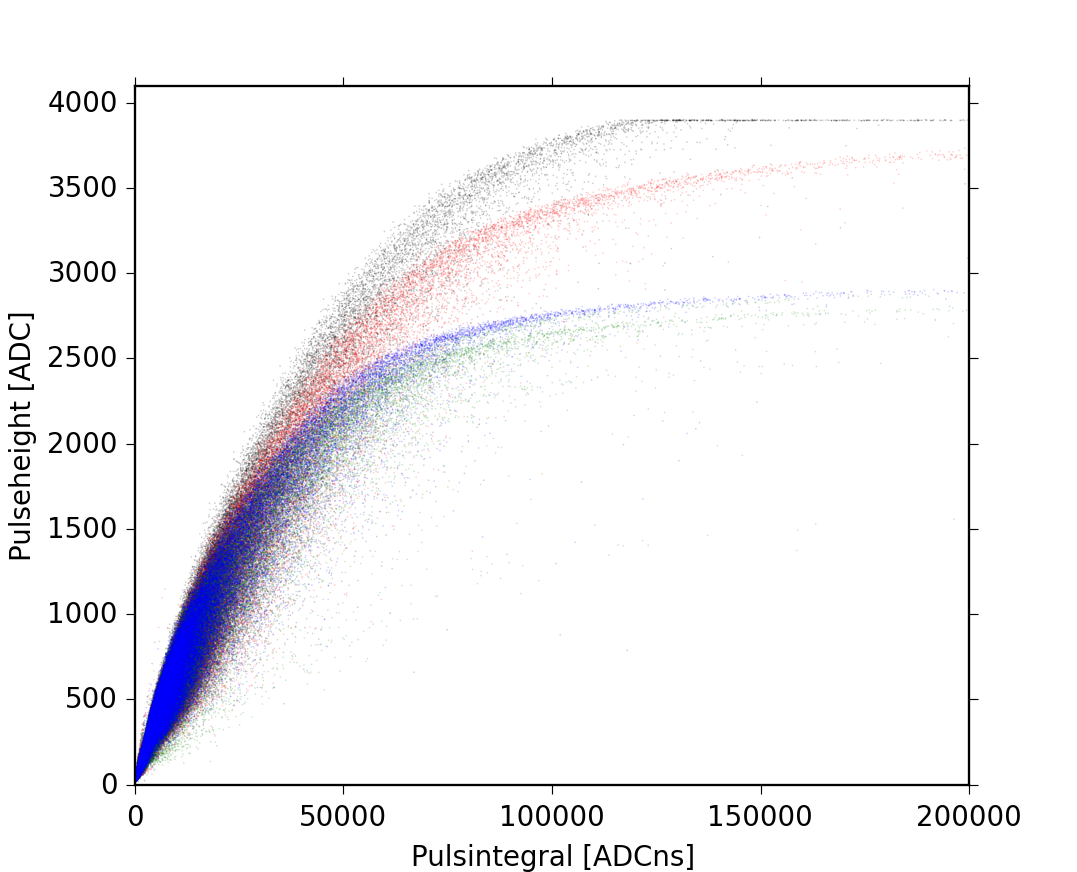
\includegraphics[width=0.6\textwidth]{plots/response/ph_vs_pi.png}
    \caption{\captitle{Pulseheight versus number of particles.}
             Indication of linearity of the \pmt.}
    \label{fig:transport_time}
\end{figure}



\subsection{Gammas}

\todo{Signals in detector from gammas}


\section{Timing}


\subsection{Fluorescence}

rise time - 0.9 ns, decay time - 2.1 ns, pulse width 2.5 ns.

\todo{deexcitation fast (2.1 ns), slow phosphorescence
      (14.2 ns), ratio?}


\subsection{Light transport and \pmt efficiency}

Similar to the model that predicts the signal transport efficiency in
the scintillator a models that calculates the transport time of these
photons has been made. Quantum efficiency of the \pmt causes not every
photon reaching the \pmt to produce a photoelectron. Multiple photons
are required for the \pmt to produce a significant signal that the
\hisparc electronics triggers. The model tracks the time at which the
15th photon producing a photoelectron reaches the \pmt. 15
photoelectrons are required for a signal of \SI{70}{\milli\volt} (high
threshold).

In the simulations for each particle within the bounds of the
scintillator a number is taken from this distribution simulate the
transport time of each particle.

\begin{figure}
    \centering
    % \usepackage{tikz}
% \usetikzlibrary{arrows}
% \usepackage{pgfplots}
% \pgfplotsset{compat=1.3}
% \usepackage[detect-family]{siunitx}
% \usepackage[eulergreek]{sansmath}
% \sisetup{text-sf=\sansmath}
% \usepackage{relsize}
%
\pgfkeysifdefined{/artist/width}
    {\pgfkeysgetvalue{/artist/width}{\defaultwidth}}
    {\def\defaultwidth{ .67\linewidth }}
%
%
\begin{sansmath}
\begin{tikzpicture}[
        font=\sffamily,
        every pin/.style={inner sep=2pt, font={\sffamily\smaller}},
        every label/.style={inner sep=2pt, font={\sffamily\smaller}},
        every pin edge/.style={<-, >=stealth', shorten <=2pt},
        pin distance=2.5ex,
    ]
    \begin{axis}[
            width=\defaultwidth,
            %
            title={  },
            %
            xlabel={ Transport time [\si{\nano\second}] },
            ylabel={ Counts },
            %
            xmin={ 1 },
            xmax={ 8 },
            ymin={ 0 },
            ymax={  },
            %
            xtick={  },
            ytick={  },
            %
            tick align=outside,
            max space between ticks=40,
            every tick/.style={},
        ]

        

        

        
            
            % Draw series plot
            \addplot[no markers,gray,const plot] coordinates {
                (1.0, 0.0)
                (1.1, 0.0)
                (1.2, 1.0)
                (1.3, 3.0)
                (1.4, 2.0)
                (1.5, 4.0)
                (1.6, 3.0)
                (1.7, 2.0)
                (1.8, 5.0)
                (1.9, 19.0)
                (2.0, 22.0)
                (2.1, 26.0)
                (2.2, 34.0)
                (2.3, 58.0)
                (2.4, 78.0)
                (2.5, 123.0)
                (2.6, 201.0)
                (2.7, 296.0)
                (2.8, 414.0)
                (2.9, 445.0)
                (3.0, 435.0)
                (3.1, 460.0)
                (3.2, 552.0)
                (3.3, 579.0)
                (3.4, 304.0)
                (3.5, 196.0)
                (3.6, 198.0)
                (3.7, 185.0)
                (3.8, 191.0)
                (3.9, 193.0)
                (4.0, 165.0)
                (4.1, 203.0)
                (4.2, 177.0)
                (4.3, 218.0)
                (4.4, 239.0)
                (4.5, 199.0)
                (4.6, 205.0)
                (4.7, 192.0)
                (4.8, 218.0)
                (4.9, 165.0)
                (5.0, 230.0)
                (5.1, 183.0)
                (5.2, 216.0)
                (5.3, 177.0)
                (5.4, 226.0)
                (5.5, 208.0)
                (5.6, 191.0)
                (5.7, 188.0)
                (5.8, 153.0)
                (5.9, 178.0)
                (6.0, 165.0)
                (6.1, 197.0)
                (6.2, 149.0)
                (6.3, 130.0)
                (6.4, 117.0)
                (6.5, 89.0)
                (6.6, 75.0)
                (6.7, 55.0)
                (6.8, 35.0)
                (6.9, 20.0)
                (7.0, 5.0)
                (7.1, 2.0)
                (7.2, 1.0)
                (7.3, 0.0)
                (7.4, 0.0)
                (7.5, 0.0)
                (7.6, 0.0)
                (7.7, 0.0)
                (7.8, 0.0)
                (7.9, 0.0)
                (8.0, 0.0)
            };
        
            
            % Draw series plot
            \addplot[no markers,black] coordinates {
                (2.5507, 0)
                (2.5507, 380.96)
                (3.4953, 380.96)
                (3.4953, 186.68)
                (6.463, 186.68)
                (6.463, 0)
            };
        

        

        

        

        

    \end{axis}
\end{tikzpicture}
\end{sansmath}
    \caption{\captitle{Signal transport time.} Time transport
             distribution in the detector.}
    \label{fig:transport_time}
\end{figure}


\subsection{\pmt transport, cable length}

The time it takes for the electron kaskade in the \pmt to go from the
front window to the anode is dependent on .. the high voltage of pmt,
position electron hits, etc? Possible second pulse from ionization of
atoms in tube.

The signal from the \pmt is transported over a \SI{30}{\meter} long
coaxial cable to the \hisparc electronics before it is digitized. To
keep the detectors in sync the cables are precisely cut to the
same length. The signal in the cables propagates at 2/3 the speed of
light or \SI{.2}{\meter\per\nano\second}. Every \SI{.2}{\meter}
difference in cable length increases the offset by a nanosecond. Kinks
and twists in the cable can also increase the propagation time.

The offset between detectors can change over time due to aging of the
\pmt, changes in the high voltage and modifications to the cables.

Offsets are determined by looking at the arrival time differences
between two detectors over many events. All events in which a signal was
detected in the reference detector (usually detector 2, because of its
central location in 4-detector stations) and in another detector are
used. Multiple events are needed to even out time differences due to the
arrival direction of the showers, transport time and the shower front.
The time difference distribution between two detectors includes a
background of accidental coincidences.

To determine the distribution of the mean offsets the distributions for
a day of data for all stations have been fit by Gaussians, the found
averages are then the distribution of the offsets. These have also been
fit by a Gaussian \figref{fig:detector_offset_distribution}. In
simulations a detector offset is drawn from this distribution and then
fixed for that detector for the entire simulation.

\todo{relative to detector 2.. different sigma if offset also given to
      detector 2?}

\begin{figure}
    \centering
    % \usepackage{tikz}
% \usetikzlibrary{arrows,external}
% \usepackage{pgfplots}
% \pgfplotsset{compat=1.3}
% \usepackage[detect-family]{siunitx}
% \usepackage[eulergreek]{sansmath}
% \sisetup{text-sf=\sansmath}
% \usepackage{relsize}
%
    \tikzsetnextfilename{ externalized-detector_offset_distribution_20140102 }
\pgfkeysifdefined{/artist/width}
    {\pgfkeysgetvalue{/artist/width}{\defaultwidth}}
    {\def\defaultwidth{ .67\linewidth }}
%
%
\begin{sansmath}
\begin{tikzpicture}[
        font=\sffamily,
        every pin/.style={inner sep=2pt, font={\sffamily\smaller}},
        every label/.style={inner sep=2pt, font={\sffamily\smaller}},
        every pin edge/.style={<-, >=stealth', shorten <=2pt},
        pin distance=2.5ex,
    ]
    \begin{axis}[
            axis background/.style={  },
            xmode=normal,
            ymode=normal,
            width=\defaultwidth,
            scale only axis,
            axis equal=false,
            %
            title={  },
            %
            xlabel={ $\Delta t$ [ns] },
            ylabel={ Occurrence },
            %
            xmin={  },
            xmax={  },
            ymin={ 0 },
            ymax={  },
            %
            xtick={  },
            ytick={  },
            %
            tick align=outside,
            max space between ticks=40,
            every tick/.style={},
            axis on top,
            point meta min={  },
            point meta max={  },
                colormap={coolwarm}{
                    rgb255(0cm)=( 59, 76,192);
                    rgb255(1cm)=( 98,130,234);
                    rgb255(2cm)=(141,176,254);
                    rgb255(3cm)=(184,208,249);
                    rgb255(4cm)=(221,221,221);
                    rgb255(5cm)=(245,196,173);
                    rgb255(6cm)=(244,154,123);
                    rgb255(7cm)=(222, 96, 77);
                    rgb255(8cm)=(180,  4, 38)},
        ]

        


    
    % Draw series plot
    \addplot[no markers,solid,const plot] coordinates {
            (-49.375, 0)
            (-48.125, 1)
            (-46.875, 0)
            (-45.625, 0)
            (-44.375, 0)
            (-43.125, 0)
            (-41.875, 0)
            (-40.625, 1)
            (-39.375, 1)
            (-38.125, 0)
            (-36.875, 0)
            (-35.625, 0)
            (-34.375, 0)
            (-33.125, 0)
            (-31.875, 0)
            (-30.625, 0)
            (-29.375, 0)
            (-28.125, 0)
            (-26.875, 0)
            (-25.625, 0)
            (-24.375, 0)
            (-23.125, 0)
            (-21.875, 0)
            (-20.625, 0)
            (-19.375, 0)
            (-18.125, 0)
            (-16.875, 0)
            (-15.625, 0)
            (-14.375, 0)
            (-13.125, 0)
            (-11.875, 0)
            (-10.625, 0)
            (-9.375, 1)
            (-8.125, 0)
            (-6.875, 1)
            (-5.625, 3)
            (-4.375, 7)
            (-3.125, 9)
            (-1.875, 11)
            (-0.625, 15)
            (0.625, 13)
            (1.875, 11)
            (3.125, 4)
            (4.375, 3)
            (5.625, 2)
            (6.875, 0)
            (8.125, 0)
            (9.375, 0)
            (10.625, 0)
            (11.875, 0)
            (13.125, 0)
            (14.375, 1)
            (15.625, 1)
            (16.875, 0)
            (18.125, 0)
            (19.375, 0)
            (20.625, 0)
            (21.875, 0)
            (23.125, 0)
            (24.375, 0)
            (25.625, 0)
            (26.875, 0)
            (28.125, 0)
            (29.375, 0)
            (30.625, 1)
            (31.875, 0)
            (33.125, 0)
            (34.375, 0)
            (35.625, 0)
            (36.875, 0)
            (38.125, 0)
            (39.375, 0)
            (40.625, 0)
            (41.875, 0)
            (43.125, 0)
            (44.375, 0)
            (45.625, 0)
            (46.875, 0)
            (48.125, 0)
    };

    
    % Draw series plot
    \addplot[no markers,gray] coordinates {
            (-48.75, 1.09919865298e-64)
            (-48.65, 2.03061331221e-64)
            (-48.55, 3.74654989725e-64)
            (-48.45, 6.90381370184e-64)
            (-48.35, 1.27057368552e-63)
            (-48.25, 2.33541411175e-63)
            (-48.15, 4.28727354586e-63)
            (-48.05, 7.86052835737e-63)
            (-47.95, 1.43938023192e-62)
            (-47.85, 2.63240422725e-62)
            (-47.75, 4.80820389252e-62)
            (-47.65, 8.77134962692e-62)
            (-47.55, 1.59809730667e-61)
            (-47.45, 2.90799240084e-61)
            (-47.35, 5.28489746223e-61)
            (-47.25, 9.59252885553e-61)
            (-47.15, 1.73893325758e-60)
            (-47.05, 3.1483714346e-60)
            (-46.95, 5.6930141555e-60)
            (-46.85, 1.0281389553e-59)
            (-46.75, 1.85444781188e-59)
            (-46.65, 3.34064762129e-59)
            (-46.55, 6.01035286714e-59)
            (-46.45, 1.07999693518e-58)
            (-46.35, 1.93819882736e-58)
            (-46.25, 3.47398053262e-58)
            (-46.15, 6.21884431865e-58)
            (-46.05, 1.11184754098e-57)
            (-45.95, 1.98533612669e-57)
            (-45.85, 3.5405937749e-57)
            (-45.75, 6.30625325864e-57)
            (-45.65, 1.12181169966e-56)
            (-45.55, 1.99306642285e-56)
            (-45.45, 3.53652580026e-56)
            (-45.35, 6.26736718542e-56)
            (-45.25, 1.10929408834e-55)
            (-45.15, 1.96092736961e-55)
            (-45.05, 3.46201996776e-55)
            (-44.95, 6.10451097853e-55)
            (-44.85, 1.0750420214e-54)
            (-44.75, 1.89083334317e-54)
            (-44.65, 3.32150044044e-54)
            (-44.55, 5.82731677528e-54)
            (-44.45, 1.02107158479e-53)
            (-44.35, 1.78688665041e-53)
            (-44.25, 3.12313723848e-53)
            (-44.15, 5.45178077099e-53)
            (-44.05, 9.50471171426e-53)
            (-43.95, 1.65498005712e-52)
            (-43.85, 2.87805991802e-52)
            (-43.75, 4.9987353941e-52)
            (-43.65, 8.67109043343e-52)
            (-43.55, 1.50224419203e-51)
            (-43.45, 2.59932510966e-51)
            (-43.35, 4.49193973631e-51)
            (-43.25, 7.75283409878e-51)
            (-43.15, 1.33641182808e-50)
            (-43.05, 2.30077092932e-50)
            (-42.95, 3.95603114863e-50)
            (-42.85, 6.79358907479e-50)
            (-42.75, 1.1651775176e-49)
            (-42.65, 1.99589719987e-49)
            (-42.55, 3.41458157108e-49)
            (-42.45, 5.8343175845e-49)
            (-42.35, 9.95625221998e-49)
            (-42.25, 1.6968949794e-48)
            (-42.15, 2.88846620044e-48)
            (-42.05, 4.91058084896e-48)
            (-41.95, 8.33780419744e-48)
            (-41.85, 1.41391652046e-47)
            (-41.75, 2.39468887291e-47)
            (-41.65, 4.05067756015e-47)
            (-41.55, 6.84320424733e-47)
            (-41.45, 1.15463463683e-46)
            (-41.35, 1.94573150408e-46)
            (-41.25, 3.27472240159e-46)
            (-41.15, 5.5045183163e-46)
            (-41.05, 9.24096663398e-46)
            (-40.95, 1.54941848763e-45)
            (-40.85, 2.59461733695e-45)
            (-40.75, 4.33941462365e-45)
            (-40.65, 7.24840132803e-45)
            (-40.55, 1.20922346155e-44)
            (-40.45, 2.0147638455e-44)
            (-40.35, 3.35270223187e-44)
            (-40.25, 5.57210213977e-44)
            (-40.15, 9.24903460485e-44)
            (-40.05, 1.53329948751e-43)
            (-39.95, 2.53869675101e-43)
            (-39.85, 4.19805297313e-43)
            (-39.75, 6.93327221982e-43)
            (-39.65, 1.14362025958e-42)
            (-39.55, 1.88399037267e-42)
            (-39.45, 3.09976498727e-42)
            (-39.35, 5.09368528338e-42)
            (-39.25, 8.3596616215e-42)
            (-39.15, 1.37024598901e-41)
            (-39.05, 2.24316712174e-41)
            (-38.95, 3.66756629363e-41)
            (-38.85, 5.9889069455e-41)
            (-38.75, 9.76720736217e-41)
            (-38.65, 1.59091325966e-40)
            (-38.55, 2.58806896849e-40)
            (-38.45, 4.20492680055e-40)
            (-38.35, 6.82329715123e-40)
            (-38.25, 1.10581730137e-39)
            (-38.15, 1.78988746498e-39)
            (-38.05, 2.89348558532e-39)
            (-37.95, 4.67164862588e-39)
            (-37.85, 7.53307459266e-39)
            (-37.75, 1.21318663134e-38)
            (-37.65, 1.95135468132e-38)
            (-37.55, 3.13471501251e-38)
            (-37.45, 5.02936509637e-38)
            (-37.35, 8.05900664159e-38)
            (-37.25, 1.28974280686e-37)
            (-37.15, 2.06147449343e-37)
            (-37.05, 3.29083469524e-37)
            (-36.95, 5.24671434297e-37)
            (-36.85, 8.35452999343e-37)
            (-36.75, 1.32864780944e-36)
            (-36.65, 2.11033294887e-36)
            (-36.55, 3.34769076342e-36)
            (-36.45, 5.30387083212e-36)
            (-36.35, 8.39254723706e-36)
            (-36.25, 1.32631872258e-35)
            (-36.15, 2.09341463846e-35)
            (-36.05, 3.30001461797e-35)
            (-35.95, 5.19552837634e-35)
            (-35.85, 8.16952543318e-35)
            (-35.75, 1.2829720277e-34)
            (-35.65, 2.01229105513e-34)
            (-35.55, 3.15222824597e-34)
            (-35.45, 4.93171267488e-34)
            (-35.35, 7.70603765717e-34)
            (-35.25, 1.20259041501e-33)
            (-35.15, 1.87437981919e-33)
            (-35.05, 2.91776769719e-33)
            (-34.95, 4.53625097499e-33)
            (-34.85, 7.04363248518e-33)
            (-34.75, 1.09231915984e-32)
            (-34.65, 1.69182588622e-32)
            (-34.55, 2.61706814033e-32)
            (-34.45, 4.0432225407e-32)
            (-34.35, 6.23869151458e-32)
            (-34.25, 9.61418838967e-32)
            (-34.15, 1.47973857231e-31)
            (-34.05, 2.27462921078e-31)
            (-33.95, 3.49212258069e-31)
            (-33.85, 5.35453298592e-31)
            (-33.75, 8.19987000133e-31)
            (-33.65, 1.25413874978e-30)
            (-33.55, 1.91574392319e-30)
            (-33.45, 2.92268881206e-30)
            (-33.35, 4.45328969877e-30)
            (-33.25, 6.77692328778e-30)
            (-33.15, 1.03000051452e-29)
            (-33.05, 1.56349164286e-29)
            (-32.95, 2.37031976155e-29)
            (-32.85, 3.58898431946e-29)
            (-32.75, 5.42737006556e-29)
            (-32.65, 8.19710615971e-29)
            (-32.55, 1.2364738466e-28)
            (-32.45, 1.86278426356e-28)
            (-32.35, 2.80280856929e-28)
            (-32.25, 4.21189526569e-28)
            (-32.15, 6.32142428562e-28)
            (-32.05, 9.47557488838e-28)
            (-31.95, 1.4185656736e-27)
            (-31.85, 2.12102884807e-27)
            (-31.75, 3.16735654964e-27)
            (-31.65, 4.72389879313e-27)
            (-31.55, 7.03651252221e-27)
            (-31.45, 1.04680935647e-26)
            (-31.35, 1.55536018389e-26)
            (-31.25, 2.3080627346e-26)
            (-31.15, 3.42071972132e-26)
            (-31.05, 5.06338119595e-26)
            (-30.95, 7.48543438606e-26)
            (-30.85, 1.10521467256e-25)
            (-30.75, 1.62978203533e-25)
            (-30.65, 2.40030075318e-25)
            (-30.55, 3.53065308671e-25)
            (-30.45, 5.18677827378e-25)
            (-30.35, 7.61015617825e-25)
            (-30.25, 1.11517418309e-24)
            (-30.15, 1.63209372238e-24)
            (-30.05, 2.38561706349e-24)
            (-29.95, 3.48264831838e-24)
            (-29.85, 5.07775520869e-24)
            (-29.75, 7.39413116067e-24)
            (-29.65, 1.07536473482e-23)
            (-29.55, 1.56198795655e-23)
            (-29.45, 2.26596304224e-23)
            (-29.35, 3.28307809933e-23)
            (-29.25, 4.7507574311e-23)
            (-29.15, 6.86590435412e-23)
            (-29.05, 9.91027925873e-23)
            (-28.95, 1.4286547398e-22)
            (-28.85, 2.05694145425e-22)
            (-28.75, 2.95780695394e-22)
            (-28.65, 4.2478675915e-22)
            (-28.55, 6.09291847268e-22)
            (-28.45, 8.72836729767e-22)
            (-28.35, 1.24880293413e-21)
            (-28.25, 1.78446509741e-21)
            (-28.15, 2.54668632327e-21)
            (-28.05, 3.62991206647e-21)
            (-27.95, 5.16737528349e-21)
            (-27.85, 7.34678199777e-21)
            (-27.75, 1.04322396045e-20)
            (-27.65, 1.47948717176e-20)
            (-27.55, 2.09555037348e-20)
            (-27.45, 2.96440991147e-20)
            (-27.35, 4.18824095091e-20)
            (-27.25, 5.90987522222e-20)
            (-27.15, 8.32871909467e-20)
            (-27.05, 1.17228003463e-19)
            (-26.95, 1.64792625385e-19)
            (-26.85, 2.31364875506e-19)
            (-26.75, 3.24422026515e-19)
            (-26.65, 4.54335307935e-19)
            (-26.55, 6.35471232409e-19)
            (-26.45, 8.87704766486e-19)
            (-26.35, 1.23849557483e-18)
            (-26.25, 1.72573305237e-18)
            (-26.15, 2.40162958834e-18)
            (-26.05, 3.33804113648e-18)
            (-25.95, 4.63372860575e-18)
            (-25.85, 6.42425474326e-18)
            (-25.75, 8.8954549449e-18)
            (-25.65, 1.2301747973e-17)
            (-25.55, 1.69909920577e-17)
            (-25.45, 2.343818074e-17)
            (-25.35, 3.22910607373e-17)
            (-25.25, 4.44318068611e-17)
            (-25.15, 6.10602935985e-17)
            (-25.05, 8.38063743142e-17)
            (-24.95, 1.14881068692e-16)
            (-24.85, 1.57279866606e-16)
            (-24.75, 2.15055744529e-16)
            (-24.65, 2.93685303363e-16)
            (-24.55, 4.00559125994e-16)
            (-24.45, 5.45637610078e-16)
            (-24.35, 7.42326929483e-16)
            (-24.25, 1.00864742486e-15)
            (-24.15, 1.36878993437e-15)
            (-24.05, 1.85518605953e-15)
            (-23.95, 2.51125833994e-15)
            (-23.85, 3.39506866615e-15)
            (-23.75, 4.58415172451e-15)
            (-23.65, 6.18190966785e-15)
            (-23.55, 8.32606077506e-15)
            (-23.45, 1.1199786635e-14)
            (-23.35, 1.50464197114e-14)
            (-23.25, 2.01887693101e-14)
            (-23.15, 2.70545160402e-14)
            (-23.05, 3.62095346987e-14)
            (-22.95, 4.84015610884e-14)
            (-22.85, 6.46173353184e-14)
            (-22.75, 8.61572782139e-14)
            (-22.65, 1.14732946592e-13)
            (-22.55, 1.52594041107e-13)
            (-22.45, 2.02693700788e-13)
            (-22.35, 2.68903329926e-13)
            (-22.25, 3.56291415823e-13)
            (-22.15, 4.71484899771e-13)
            (-22.05, 6.23136897788e-13)
            (-21.95, 8.22531233457e-13)
            (-21.85, 1.08436272152e-12)
            (-21.75, 1.42774290335e-12)
            (-21.65, 1.87749458008e-12)
            (-21.55, 2.4658157616e-12)
            (-21.45, 3.23441548183e-12)
            (-21.35, 4.23725148416e-12)
            (-21.25, 5.54403450221e-12)
            (-21.15, 7.2447075489e-12)
            (-21.05, 9.45516351192e-12)
            (-20.95, 1.23245332013e-11)
            (-20.85, 1.60444622245e-11)
            (-20.75, 2.08609028975e-11)
            (-20.65, 2.70890820445e-11)
            (-20.55, 3.51324733955e-11)
            (-20.45, 4.55068122321e-11)
            (-20.35, 5.88704496096e-11)
            (-20.25, 7.60626657094e-11)
            (-20.15, 9.81519610973e-11)
            (-20.05, 1.26496838496e-10)
            (-19.95, 1.62822197592e-10)
            (-19.85, 2.09315217471e-10)
            (-19.75, 2.68745527191e-10)
            (-19.65, 3.44615603146e-10)
            (-19.55, 4.41348728556e-10)
            (-19.45, 5.64523561842e-10)
            (-19.35, 7.21166454073e-10)
            (-19.25, 9.20115212496e-10)
            (-19.15, 1.17247112476e-09)
            (-19.05, 1.4921598536e-09)
            (-18.95, 1.89662642441e-09)
            (-18.85, 2.4076951246e-09)
            (-18.75, 3.05263191358e-09)
            (-18.65, 3.86545514104e-09)
            (-18.55, 4.88855027037e-09)
            (-18.45, 6.17465623581e-09)
            (-18.35, 7.78930541935e-09)
            (-18.25, 9.81381648058e-09)
            (-18.15, 1.23489599564e-08)
            (-18.05, 1.55194413095e-08)
            (-17.95, 1.94793756979e-08)
            (-17.85, 2.44189640471e-08)
            (-17.75, 3.05726220553e-08)
            (-17.65, 3.82288637605e-08)
            (-17.55, 4.77423006331e-08)
            (-17.45, 5.95481874539e-08)
            (-17.35, 7.4180029376e-08)
            (-17.25, 9.22908627037e-08)
            (-17.15, 1.14678937572e-07)
            (-17.05, 1.4231866673e-07)
            (-16.95, 1.76397864325e-07)
            (-16.85, 2.18362485756e-07)
            (-16.75, 2.69970298528e-07)
            (-16.65, 3.33355169674e-07)
            (-16.55, 4.11103953065e-07)
            (-16.45, 5.06348306358e-07)
            (-16.35, 6.22874169367e-07)
            (-16.25, 7.65252101464e-07)
            (-16.15, 9.38992214226e-07)
            (-16.05, 1.15072805701e-06)
            (-15.95, 1.40843452887e-06)
            (-15.85, 1.72168571279e-06)
            (-15.75, 2.10195947144e-06)
            (-15.65, 2.56299672347e-06)
            (-15.55, 3.12122455203e-06)
            (-15.45, 3.79625370258e-06)
            (-15.35, 4.61146262425e-06)
            (-15.25, 5.59468202196e-06)
            (-15.15, 6.77899593811e-06)
            (-15.05, 8.20367769987e-06)
            (-14.95, 9.91528167905e-06)
            (-14.85, 1.19689147463e-05)
            (-14.75, 1.44297145925e-05)
            (-14.65, 1.73745657697e-05)
            (-14.55, 2.08940884128e-05)
            (-14.45, 2.50949391703e-05)
            (-14.35, 3.01024689454e-05)
            (-14.25, 3.60637876601e-05)
            (-14.15, 4.31512924511e-05)
            (-14.05, 5.15667225187e-05)
            (-13.95, 6.15458113326e-05)
            (-13.85, 7.33636150712e-05)
            (-13.75, 8.73406050929e-05)
            (-13.65, 0.000103849621917)
            (-13.55, 0.000123323798689)
            (-13.45, 0.000146265573404)
            (-13.35, 0.000173256921334)
            (-13.25, 0.000204970952105)
            (-13.15, 0.000242185029722)
            (-13.05, 0.000285795588577)
            (-12.95, 0.000336834833941)
            (-12.85, 0.000396489531792)
            (-12.75, 0.000466122109788)
            (-12.65, 0.000547294308875)
            (-12.55, 0.00064179364316)
            (-12.45, 0.00075166294429)
            (-12.35, 0.000879233285357)
            (-12.25, 0.00102716059828)
            (-12.15, 0.00119846631724)
            (-12.05, 0.00139658239922)
            (-11.95, 0.00162540108996)
            (-11.85, 0.00188932982052)
            (-11.75, 0.00219335163447)
            (-11.65, 0.00254309155912)
            (-11.55, 0.0029448893449)
            (-11.45, 0.0034058790054)
            (-11.35, 0.00393407559498)
            (-11.25, 0.00453846966177)
            (-11.15, 0.0052291298097)
            (-11.05, 0.00601731379441)
            (-10.95, 0.00691558856204)
            (-10.85, 0.00793795961849)
            (-10.75, 0.00910001008673)
            (-10.65, 0.0104190497721)
            (-10.55, 0.0119142745086)
            (-10.45, 0.0136069360022)
            (-10.35, 0.0155205223197)
            (-10.25, 0.0176809490932)
            (-10.15, 0.0201167614192)
            (-10.05, 0.0228593463264)
            (-9.95, 0.025943155573)
            (-9.85, 0.0294059383989)
            (-9.75, 0.0332889837187)
            (-9.65, 0.0376373710796)
            (-9.55, 0.0425002295362)
            (-9.45, 0.0479310034096)
            (-9.35, 0.0539877236945)
            (-9.25, 0.0607332836685)
            (-9.15, 0.06823571703)
            (-9.05, 0.0765684766568)
            (-8.95, 0.0858107118309)
            (-8.85, 0.0960475415227)
            (-8.75, 0.107370321069)
            (-8.65, 0.119876899314)
            (-8.55, 0.133671863035)
            (-8.45, 0.148866765182)
            (-8.35, 0.165580333254)
            (-8.25, 0.183938653846)
            (-8.15, 0.204075329196)
            (-8.05, 0.226131601357)
            (-7.95, 0.250256439399)
            (-7.85, 0.27660658491)
            (-7.75, 0.305346550946)
            (-7.65, 0.336648569453)
            (-7.55, 0.370692482166)
            (-7.45, 0.407665569985)
            (-7.35, 0.44776231587)
            (-7.25, 0.491184096418)
            (-7.15, 0.538138797455)
            (-7.05, 0.588840349209)
            (-6.95, 0.643508176947)
            (-6.85, 0.702366563345)
            (-6.75, 0.765643919301)
            (-6.65, 0.833571960462)
            (-6.55, 0.906384787322)
            (-6.45, 0.984317867478)
            (-6.35, 1.06760691935)
            (-6.25, 1.15648669761)
            (-6.15, 1.25118968129)
            (-6.05, 1.35194466686)
            (-5.95, 1.4589752692)
            (-5.85, 1.57249833483)
            (-5.75, 1.69272227273)
            (-5.65, 1.81984530933)
            (-5.55, 1.95405367546)
            (-5.45, 2.09551973415)
            (-5.35, 2.24440005971)
            (-5.25, 2.40083347918)
            (-5.15, 2.56493908912)
            (-5.05, 2.73681426118)
            (-4.95, 2.91653265128)
            (-4.85, 3.10414222835)
            (-4.75, 3.29966333907)
            (-4.65, 3.50308682618)
            (-4.55, 3.71437221847)
            (-4.45, 3.93344601084)
            (-4.35, 4.1602000537)
            (-4.25, 4.39449007044)
            (-4.15, 4.63613432229)
            (-4.05, 4.88491243927)
            (-3.95, 5.14056443578)
            (-3.85, 5.40278992843)
            (-3.75, 5.67124757317)
            (-3.65, 5.94555473746)
            (-3.55, 6.22528742203)
            (-3.45, 6.50998044518)
            (-3.35, 6.79912790101)
            (-3.25, 7.09218390074)
            (-3.15, 7.38856360448)
            (-3.05, 7.68764454837)
            (-2.95, 7.98876826953)
            (-2.85, 8.29124222876)
            (-2.75, 8.5943420283)
            (-2.65, 8.89731391909)
            (-2.55, 9.19937758922)
            (-2.45, 9.49972922242)
            (-2.35, 9.79754481267)
            (-2.25, 10.0919837182)
            (-2.15, 10.3821924353)
            (-2.05, 10.6673085701)
            (-1.95, 10.946464984)
            (-1.85, 11.2187940853)
            (-1.75, 11.4834322392)
            (-1.65, 11.7395242649)
            (-1.55, 11.986227988)
            (-1.45, 12.2227188143)
            (-1.35, 12.4481942912)
            (-1.25, 12.6618786209)
            (-1.15, 12.8630270911)
            (-1.05, 13.050930387)
            (-0.949999999999, 13.2249187503)
            (-0.849999999999, 13.3843659507)
            (-0.749999999999, 13.5286930375)
            (-0.649999999999, 13.6573718396)
            (-0.549999999999, 13.7699281847)
            (-0.449999999999, 13.865944809)
            (-0.349999999999, 13.9450639343)
            (-0.249999999999, 14.0069894887)
            (-0.149999999999, 14.0514889525)
            (-0.0499999999993, 14.0783948125)
            (0.0500000000007, 14.0876056126)
            (0.150000000001, 14.0790865912)
            (0.250000000001, 14.0528698996)
            (0.350000000001, 14.0090544001)
            (0.450000000001, 13.9478050447)
            (0.550000000001, 13.8693518407)
            (0.650000000001, 13.7739884116)
            (0.750000000001, 13.6620701664)
            (0.850000000001, 13.5340120933)
            (0.950000000001, 13.3902861959)
            (1.05, 13.2314185964)
            (1.15, 13.0579863271)
            (1.25, 12.870613842)
            (1.35, 12.6699692737)
            (1.45, 12.4567604699)
            (1.55, 12.2317308415)
            (1.65, 11.9956550551)
            (1.75, 11.7493346075)
            (1.85, 11.4935933138)
            (1.95, 11.2292727483)
            (2.05, 10.9572276697)
            (2.15, 10.6783214675)
            (2.25, 10.3934216624)
            (2.35, 10.1033954921)
            (2.45, 9.80910561443)
            (2.55, 9.51140595572)
            (2.65, 9.2111377319)
            (2.75, 8.90912566642)
            (2.85, 8.60617442732)
            (2.95, 8.30306530297)
            (3.05, 8.00055313327)
            (3.15, 7.69936351043)
            (3.25, 7.40019026058)
            (3.35, 7.10369321459)
            (3.45, 6.81049627378)
            (3.55, 6.52118577332)
            (3.65, 6.2363091435)
            (3.75, 5.95637386654)
            (3.85, 5.68184672401)
            (3.95, 5.41315332772)
            (4.05, 5.15067792497)
            (4.15, 4.89476346673)
            (4.25, 4.645711926)
            (4.35, 4.40378485182)
            (4.45, 4.16920414317)
            (4.55, 3.94215302581)
            (4.65, 3.72277721447)
            (4.75, 3.51118624191)
            (4.85, 3.30745493593)
            (4.95, 3.11162502548)
            (5.05, 2.92370685658)
            (5.15, 2.74368119921)
            (5.25, 2.57150112653)
            (5.35, 2.4070939484)
            (5.45, 2.25036318154)
            (5.55, 2.10119053989)
            (5.65, 1.95943792917)
            (5.75, 1.82494943084)
            (5.85, 1.69755326177)
            (5.95, 1.57706369695)
            (6.05, 1.46328294372)
            (6.15, 1.35600295732)
            (6.25, 1.25500718874)
            (6.35, 1.16007225697)
            (6.45, 1.07096953907)
            (6.55, 0.987466672734)
            (6.65, 0.909328966896)
            (6.75, 0.836320717332)
            (6.85, 0.768206425082)
            (6.95, 0.704751916568)
            (7.05, 0.645725365179)
            (7.15, 0.59089821497)
            (7.25, 0.540046007861)
            (7.35, 0.492949116456)
            (7.45, 0.449393385192)
            (7.55, 0.409170683077)
            (7.65, 0.372079371739)
            (7.75, 0.337924692898)
            (7.85, 0.30651907966)
            (7.95, 0.277682396325)
            (8.05, 0.251242111506)
            (8.15, 0.227033409543)
            (8.25, 0.204899245185)
            (8.35, 0.184690346569)
            (8.45, 0.166265171436)
            (8.55, 0.149489821467)
            (8.65, 0.134237919472)
            (8.75, 0.120390454019)
            (8.85, 0.1078355959)
            (8.95, 0.0964684906114)
            (9.05, 0.0861910308163)
            (9.15, 0.0769116124863)
            (9.25, 0.0685448781942)
            (9.35, 0.0610114507516)
            (9.45, 0.0542376601309)
            (9.55, 0.0481552663476)
            (9.65, 0.0427011807196)
            (9.75, 0.0378171876676)
            (9.85, 0.0334496689745)
            (9.95, 0.0295493321851)
            (10.05, 0.0260709446028)
            (10.15, 0.0229730741251)
            (10.25, 0.0202178379593)
            (10.35, 0.0177706600746)
            (10.45, 0.0156000380697)
            (10.55, 0.0136773199801)
            (10.65, 0.0119764914008)
            (10.75, 0.0104739731723)
            (10.85, 0.00914842975766)
            (10.95, 0.00798058833598)
            (11.05, 0.00695306854593)
            (11.15, 0.00605022273346)
            (11.25, 0.00525798649)
            (11.35, 0.00456373921025)
            (11.45, 0.00395617435134)
            (11.55, 0.00342517903687)
            (11.65, 0.00296172261962)
            (11.75, 0.00255775379424)
            (11.85, 0.0022061058359)
            (11.95, 0.00190040953126)
            (12.05, 0.00163501336424)
            (12.15, 0.00140491051928)
            (12.25, 0.0012056722696)
            (12.35, 0.00103338732586)
            (12.45, 0.000884606731371)
            (12.55, 0.000756293903102)
            (12.65, 0.000645779433055)
            (12.75, 0.000550720280639)
            (12.85, 0.000469063004527)
            (12.95, 0.000399010700593)
            (13.05, 0.000338993331291)
            (13.15, 0.000287641150695)
            (13.25, 0.000243760948236)
            (13.35, 0.000206314852782)
            (13.45, 0.000174401456883)
            (13.55, 0.000147239038677)
            (13.65, 0.000124150675972)
            (13.75, 0.000104551063369)
            (13.85, 8.79348588068e-05)
            (13.95, 7.38664006674e-05)
            (14.05, 6.19706504742e-05)
            (14.15, 5.19252292464e-05)
            (14.25, 4.34534277744e-05)
            (14.35, 3.63180824177e-05)
            (14.45, 3.03162185519e-05)
            (14.55, 2.52743735042e-05)
            (14.65, 2.10445197665e-05)
            (14.75, 1.75005174763e-05)
            (14.85, 1.45350326649e-05)
            (14.95, 1.20568646099e-05)
            (15.05, 9.98863184931e-06)
            (15.15, 8.26477204739e-06)
            (15.25, 6.82981599402e-06)
            (15.35, 5.63690060945e-06)
            (15.45, 4.64648994806e-06)
            (15.55, 3.82527689314e-06)
            (15.65, 3.14524153903e-06)
            (15.75, 2.58284520543e-06)
            (15.85, 2.11834165177e-06)
            (15.95, 1.73518938729e-06)
            (16.05, 1.41955103447e-06)
            (16.15, 1.1598675248e-06)
            (16.25, 9.464965113e-07)
            (16.35, 7.71405794544e-07)
            (16.45, 6.27913798173e-07)
            (16.55, 5.10470215084e-07)
            (16.65, 4.14470893939e-07)
            (16.75, 3.36101862537e-07)
            (16.85, 2.72208104283e-07)
            (16.95, 2.20183328905e-07)
            (17.05, 1.77877520229e-07)
            (17.15, 1.43519512268e-07)
            (17.25, 1.15652249318e-07)
            (17.35, 9.30787341303e-08)
            (17.45, 7.48169678394e-08)
            (17.55, 6.00624424353e-08)
            (17.65, 4.81569668054e-08)
            (17.75, 3.85627956836e-08)
            (17.85, 3.08411915346e-08)
            (17.95, 2.46346862861e-08)
            (18.05, 1.96524262055e-08)
            (18.15, 1.56580819901e-08)
            (18.25, 1.24598898203e-08)
            (18.35, 9.90245988304e-09)
            (18.45, 7.86004860899e-09)
            (18.55, 6.2310411962e-09)
            (18.65, 4.93343333293e-09)
            (18.75, 3.90113658191e-09)
            (18.85, 3.08096168792e-09)
            (18.95, 2.43015900662e-09)
            (19.05, 1.9144160823e-09)
            (19.15, 1.5062297728e-09)
            (19.25, 1.18358478091e-09)
            (19.35, 9.28882470316e-10)
            (19.45, 7.28073815667e-10)
            (19.55, 5.69958596478e-10)
            (19.65, 4.45619774761e-10)
            (19.75, 3.47967635246e-10)
            (19.85, 2.71372914682e-10)
            (19.95, 2.11371971039e-10)
            (20.05, 1.64430185116e-10)
            (20.15, 1.27752363839e-10)
            (20.25, 9.91310244451e-11)
            (20.35, 7.68251637097e-11)
            (20.45, 5.94635242266e-11)
            (20.55, 4.59675170775e-11)
            (20.65, 3.5489893633e-11)
            (20.75, 2.73660174702e-11)
            (20.85, 2.1075202322e-11)
            (20.95, 1.62100799087e-11)
            (21.05, 1.24523640636e-11)
            (21.15, 9.55370250764e-12)
            (21.25, 7.3205695057e-12)
            (21.35, 5.60236336876e-12)
            (21.45, 4.2820420668e-12)
            (21.55, 3.26876602855e-12)
            (21.65, 2.49212597985e-12)
            (21.75, 1.89762065985e-12)
            (21.85, 1.44311871168e-12)
            (21.95, 1.09609441845e-12)
            (22.05, 8.31471035655e-13)
            (22.15, 6.29940505449e-13)
            (22.25, 4.76656143076e-13)
            (22.35, 3.60216917076e-13)
            (22.45, 2.71879376931e-13)
            (22.55, 2.04947052832e-13)
            (22.65, 1.54298015171e-13)
            (22.75, 1.16019837287e-13)
            (22.85, 8.71279338124e-14)
            (22.95, 6.53485309075e-14)
            (23.05, 4.89516677839e-14)
            (23.15, 3.66228727043e-14)
            (23.25, 2.73646925181e-14)
            (23.35, 2.04212343036e-14)
            (23.45, 1.52204206198e-14)
            (23.55, 1.13298607225e-14)
            (23.65, 8.42317334483e-15)
            (23.75, 6.25432083675e-15)
            (23.85, 4.63807561131e-15)
            (23.95, 3.43517402458e-15)
            (24.05, 2.54104825488e-15)
            (24.15, 1.87728552834e-15)
            (24.25, 1.38516338369e-15)
            (24.35, 1.02076300905e-15)
            (24.45, 7.51280462418e-16)
            (24.55, 5.52245920977e-16)
            (24.65, 4.05430287327e-16)
            (24.75, 2.97271388819e-16)
            (24.85, 2.17692409123e-16)
            (24.95, 1.5921600024e-16)
            (25.05, 1.16300982614e-16)
            (25.15, 8.48463783087e-17)
            (25.25, 6.18210653081e-17)
            (25.35, 4.49876088711e-17)
            (25.45, 3.26965994679e-17)
            (25.55, 2.37337035997e-17)
            (25.65, 1.72060702589e-17)
            (25.75, 1.24580801351e-17)
            (25.85, 9.00894216249e-18)
            (25.95, 6.50653436537e-18)
            (26.05, 4.69330639788e-18)
            (26.15, 3.38112586367e-18)
            (26.25, 2.4327474084e-18)
            (26.35, 1.74817920474e-18)
            (26.45, 1.25466600674e-18)
            (26.55, 8.99339283327e-19)
            (26.65, 6.43831537983e-19)
            (26.75, 4.60335194823e-19)
            (26.85, 3.28722449091e-19)
            (26.95, 2.34443285122e-19)
            (27.05, 1.66993467712e-19)
            (27.15, 1.18799446872e-19)
            (27.25, 8.4407804572e-20)
            (27.35, 5.98968579583e-20)
            (27.45, 4.24501010056e-20)
            (27.55, 3.00473838758e-20)
            (27.65, 2.12416306694e-20)
            (27.75, 1.49976181505e-20)
            (27.85, 1.05757209009e-20)
            (27.95, 7.44819298106e-21)
            (28.05, 5.23896033906e-21)
            (28.15, 3.68037906197e-21)
            (28.25, 2.58222001125e-21)
            (28.35, 1.80945248816e-21)
            (28.45, 1.26635181234e-21)
            (28.55, 8.85145812128e-22)
            (28.65, 6.17914678758e-22)
            (28.75, 4.30819602682e-22)
            (28.85, 2.99996128501e-22)
            (28.95, 2.08635926551e-22)
            (29.05, 1.44915817184e-22)
            (29.15, 1.00530012366e-22)
            (29.25, 6.96512527879e-23)
            (29.35, 4.81964864566e-23)
            (29.45, 3.33085000925e-23)
            (29.55, 2.29904792455e-23)
            (29.65, 1.58487210959e-23)
            (29.75, 1.09117315194e-23)
            (29.85, 7.50319737954e-24)
            (29.95, 5.15290719914e-24)
            (30.05, 3.53436600746e-24)
            (30.15, 2.42116268885e-24)
            (30.25, 1.65649326383e-24)
            (30.35, 1.13190147588e-24)
            (30.45, 7.72468589143e-25)
            (30.55, 5.26509585005e-25)
            (30.65, 3.58414016634e-25)
            (30.75, 2.43678346783e-25)
            (30.85, 1.65463476232e-25)
            (30.95, 1.12212334942e-25)
            (31.05, 7.60032747389e-26)
            (31.15, 5.14135108393e-26)
            (31.25, 3.47356530261e-26)
            (31.35, 2.34383440641e-26)
            (31.45, 1.57954365373e-26)
            (31.55, 1.06313787694e-26)
            (31.65, 7.14662180414e-27)
            (31.75, 4.7980554132e-27)
            (31.85, 3.21723636678e-27)
            (31.95, 2.15453686561e-27)
            (32.05, 1.44104698277e-27)
            (32.15, 9.6262159862e-28)
            (32.25, 6.42223678486e-28)
            (32.35, 4.27927578485e-28)
            (32.45, 2.84778690817e-28)
            (32.55, 1.89277047403e-28)
            (32.65, 1.25643974683e-28)
            (32.75, 8.32987781583e-29)
            (32.85, 5.51555025699e-29)
            (32.95, 3.64747489785e-29)
            (33.05, 2.40906782773e-29)
            (33.15, 1.58912841908e-29)
            (33.25, 1.04694100884e-29)
            (33.35, 6.88872232287e-30)
            (33.45, 4.52697813937e-30)
            (33.55, 2.97119643961e-30)
            (33.65, 1.94763506608e-30)
            (33.75, 1.27507888762e-30)
            (33.85, 8.33719146235e-31)
            (33.95, 5.4444717145e-31)
            (34.05, 3.5509533522e-31)
            (34.15, 2.31306287906e-31)
            (34.25, 1.50481517198e-31)
            (34.35, 9.77759702149e-32)
            (34.45, 6.34503989975e-32)
            (34.55, 4.1123477384e-32)
            (34.65, 2.66194179846e-32)
            (34.75, 1.72091940065e-32)
            (34.85, 1.11115784298e-32)
            (34.95, 7.16546257404e-33)
            (35.05, 4.61493893123e-33)
            (35.15, 2.96852653565e-33)
            (35.25, 1.9070811036e-33)
            (35.35, 1.22363147874e-33)
            (35.45, 7.84125124538e-34)
            (35.55, 5.018493299e-34)
            (35.65, 3.20785388394e-34)
            (35.75, 2.04790147256e-34)
            (35.85, 1.30574024182e-34)
            (35.95, 8.3149141594e-35)
            (36.05, 5.28825028803e-35)
            (36.15, 3.35907332327e-35)
            (36.25, 2.13098413586e-35)
            (36.35, 1.35018786329e-35)
            (36.45, 8.54400381465e-36)
            (36.55, 5.39985275938e-36)
            (36.65, 3.4084399943e-36)
            (36.75, 2.1487339114e-36)
            (36.85, 1.35289120585e-36)
            (36.95, 8.50739034672e-37)
            (37.05, 5.34297444468e-37)
            (37.15, 3.35137545288e-37)
            (37.25, 2.09950214293e-37)
            (37.35, 1.31359900458e-37)
            (37.45, 8.20847631915e-38)
            (37.55, 5.12289599684e-38)
            (37.65, 3.19316807849e-38)
            (37.75, 1.98783928681e-38)
            (37.85, 1.23593038843e-38)
            (37.95, 7.67467515343e-39)
            (38.05, 4.75969631565e-39)
            (38.15, 2.94816466552e-39)
            (38.25, 1.82380112751e-39)
            (38.35, 1.12682499923e-39)
            (38.45, 6.95326397956e-40)
            (38.55, 4.28523074617e-40)
            (38.65, 2.63762443494e-40)
            (38.75, 1.62145519746e-40)
            (38.85, 9.95520481247e-41)
            (38.95, 6.10448029388e-41)
            (39.05, 3.73852632732e-41)
            (39.15, 2.28668025186e-41)
            (39.25, 1.39689476386e-41)
            (39.35, 8.52266049176e-42)
            (39.45, 5.19325846396e-42)
            (39.55, 3.16051559376e-42)
            (39.65, 1.92100806346e-42)
            (39.75, 1.16614804548e-42)
            (39.85, 7.07019578275e-43)
            (39.95, 4.28116969037e-43)
            (40.05, 2.58908730062e-43)
            (40.15, 1.5638107617e-43)
            (40.25, 9.43354555439e-44)
            (40.35, 5.68354044695e-44)
            (40.45, 3.41992206735e-44)
            (40.55, 2.0552597379e-44)
            (40.65, 1.23358894907e-44)
            (40.75, 7.3948177713e-45)
            (40.85, 4.42728757823e-45)
            (40.95, 2.64728829852e-45)
            (41.05, 1.58094950031e-45)
            (41.15, 9.42948569096e-46)
            (41.25, 5.61708847481e-46)
            (41.35, 3.3418563188e-46)
            (41.45, 1.98571782103e-46)
            (41.55, 1.17842119121e-46)
            (41.65, 6.98452384669e-47)
            (41.75, 4.13453160178e-47)
            (41.85, 2.44438200322e-47)
            (41.95, 1.44332817629e-47)
            (42.05, 8.51166167421e-48)
            (42.15, 5.01322118331e-48)
            (42.25, 2.94898545138e-48)
            (42.35, 1.73253351431e-48)
            (42.45, 1.01658549637e-48)
            (42.55, 5.95743653915e-49)
            (42.65, 3.48680926049e-49)
            (42.75, 2.03821600351e-49)
            (42.85, 1.189941125e-49)
            (42.95, 6.93831466138e-50)
            (43.05, 4.04050603526e-50)
            (43.15, 2.35001577927e-50)
            (43.25, 1.36508296615e-50)
            (43.35, 7.91955113044e-51)
            (43.45, 4.58875992854e-51)
            (43.55, 2.6554819749e-51)
            (43.65, 1.53477469128e-51)
            (43.75, 8.85929474401e-52)
            (43.85, 5.10748291878e-52)
            (43.95, 2.94081662996e-52)
            (44.05, 1.69115034616e-52)
            (44.15, 9.71291845448e-53)
            (44.25, 5.5714792433e-53)
            (44.35, 3.19186519924e-53)
            (44.45, 1.82629872956e-53)
            (44.55, 1.04364390913e-53)
            (44.65, 5.9564310545e-54)
            (44.75, 3.39526085274e-54)
            (44.85, 1.93291796928e-54)
            (44.95, 1.09902343048e-54)
            (45.05, 6.24099349395e-55)
            (45.15, 3.53959651472e-55)
            (45.25, 2.00496611994e-55)
            (45.35, 1.13426248492e-55)
            (45.45, 6.40875027074e-56)
            (45.55, 3.61648259932e-56)
            (45.65, 2.03822752133e-56)
            (45.75, 1.14728731933e-56)
            (45.85, 6.44978111126e-57)
            (45.95, 3.62135423753e-57)
            (46.05, 2.0307211537e-57)
            (46.15, 1.1373203944e-57)
            (46.25, 6.36163300621e-58)
            (46.35, 3.55391999498e-58)
            (46.45, 1.98289598113e-58)
            (46.55, 1.10495723216e-58)
            (46.65, 6.14956300696e-59)
            (46.75, 3.41819073604e-59)
            (46.85, 1.89758649397e-59)
            (46.95, 1.05210750588e-59)
            (47.05, 5.82601914932e-60)
            (47.15, 3.22208465873e-60)
            (47.25, 1.77973457254e-60)
            (47.35, 9.81808476706e-61)
            (47.45, 5.40943078537e-61)
            (47.55, 2.97666259231e-61)
            (47.65, 1.63591562952e-61)
            (47.75, 8.97936125138e-62)
            (47.85, 4.92247180358e-62)
            (47.95, 2.69509625547e-62)
            (48.05, 1.47373220687e-62)
            (48.15, 8.04852169835e-63)
            (48.25, 4.39002419997e-63)
            (48.35, 2.39150316452e-63)
            (48.45, 1.30115266625e-63)
            (48.55, 7.07031564306e-64)
            (48.65, 3.83709542443e-64)
    };

    \node[,
          below left=2pt
        ]
        at (rel axis cs:1,1)
        { $\mu$: 0.05, $\sigma$: 2.82 };

    \end{axis}
\end{tikzpicture}
\end{sansmath}
    \caption{\captitle{Detector offset distribution.} In black the mean
             detector offsets for all detectors relative to detector 2
             in each station are plotted. The gray line is a fit
             Gaussian. The mean of the offset distribution is
             \SI{0}{\nano\second} and the sigma is
             \SI{2.7}{\nano\second}.}
    \label{fig:detector_offset_distribution}
\end{figure}

